%Author: Marius
\label{sec:fixed_data}
\textit{Author: Marius Schidlack} \\
After working with our fake data streams for some time, we were provided with some real data by BMW. The data was presented in two different formats: Flowlogs and Metrics. They contained network traffic information  starting from December 21, 2018. 
Flowlogs contain raw information about network traffic, e.g. which IP-adress made a request to which server at what time along with other details.

In this section, we will focus on how we used the Metrics files. The Metrics already accumulate the raw network traffic data from the Flowlogs and only contain information about the number of requests. More specifically, they contain the number of successful requests (with HTTP-Code 200) and failed requests (HTTP-Code 4xx and 5xx) at a certain time. Although the files were named \textit{output-mass.json}, they were not correctly encoded in JSON format. An example entry from one of the files can be seen in \ref{lst:metrics_example}.

\begin{minipage}{\linewidth}
\begin{lstlisting}[caption={Example entry from metrics data},label={lst:metrics_example}]
{
    [...]
    'response-code-4xx': {
    [...]
        'Datapoints': [
            {'Timestamp': datetime.datetime(2018, 12, 15, 11, 20, tzinfo=tzlocal()), 
            'SampleCount': 6.0, 
            'Unit': 'None'
            }
        ]
    }
}
\end{lstlisting}
\end{minipage}

For this reason (invalid JSON format) we had to write a custom python script to parse the data (i.e. to read the data from the files and load them into python objects). Once all the files are parsed, we take the \textit{SampleCount} values for each entry, and sort them into buckets according to their \textit{Timestamp}. For the time being, we did not differentiate between successful or failed requests, however, this might be a useful thing to do in the future. The buckets were chosen to be of 5 minute granularity in the final product, however we also experimented with 1 minute buckets.
\begin{figure}[h]
    \centering
    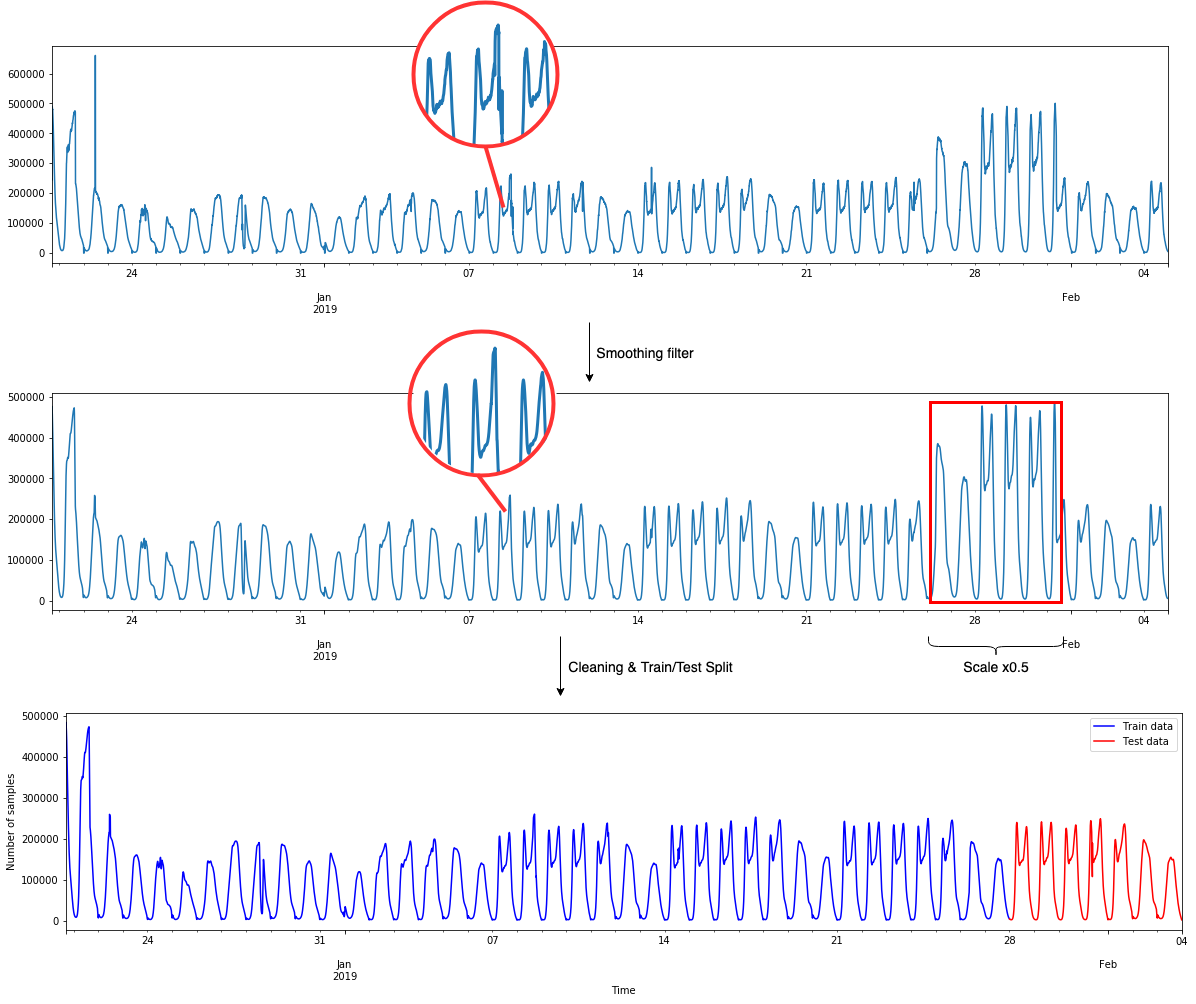
\includegraphics[width=1\textwidth]{images/data_preprocessing.png}
    \caption{Data preprocessing pipeline}
    \label{fig:data_preprocessing}
\end{figure}
\afterpage{\FloatBarrier}
A smaller bucket size means higher responsiveness in a real time anomaly detection model, since in order to react to incoming data, we have to wait until the current bucket is full. On the other hand, if the bucket size gets too small, the machine learning model might get vulnerable to noise in the data. Larger buckets means less number of buckets and compress the training data which allows to train the model faster. Furthermore this can make the model more robust to noisy data. \\
Next, we summed up the values in every bucket to obtain the raw time series, which can be seen in figure \ref{fig:data_preprocessing} in the first graph. 
\subsubsection{Preprocessing and Cleaning}
We noticed that the data is still very noisy and contains some impurities. For example, the data between the 26th and the 31st of January was scaled up by a factor of two for unknown reasons (see red box in the second graph in figure \ref{fig:data_preprocessing}).
We reduced the noise by applying a smoothing convolution to the data, and scaled down the aforementioned scaled up time interval (cf. fig. \ref{fig:data_preprocessing}).
One might argue that in time series data, the value of one point in time is highly correlated to the previous ones. Smoothing the time series exploits this property to get rid of sudden and unexpected jumps in the training data, or in other words, we reduce outliers and make training of our machine learning models more robust.
Finally, we separated one week of data and defined it as out test set.
\subsubsection{Exporting for Machine Learning Models}
For further use with the Machine Learning models described later, the data had to exported in different formats. For the Random Cut Forest and the Mean Predictor, the data can be provided in a simple CSV format with \textit{Timestamp} and \textit{Value}. The DeepAR Model however requires a more complex format which is described in more detail in chapter \pageref{ch:deepar}.

\subsubsection{Advantages and Disadvantages}
While extracting the data from the Metrics files is convenient and simple, this approach has drawbacks: we have no control over how the Metrics files are accumulated. In order to obtain full control over the data stream, one must work with the raw Flowlogs files. An approach that utilizes the Flowlogs data from scratch is described in section \ref{sec:real_time_anomaly_detection}.

